\section{Protecting DeFi Values in a (Soon to be) Regulated World}\label{sec:introduction}

DeFi is growing at an unprecedented rate.\\

At the start of 2020, the ecosystem’s Total Locked Value (TVL) sat at \$630 million. Within 12 months, that figure rose to \$18 billion. By the start of 2022, DeFi’s TVL had hit \$240 billion. That’s a Compound Annual Growth Rate (CAGR) of 1,851\% over two years.\\\\

\begin{figure}[h]
  \begin{center}
    \centering
    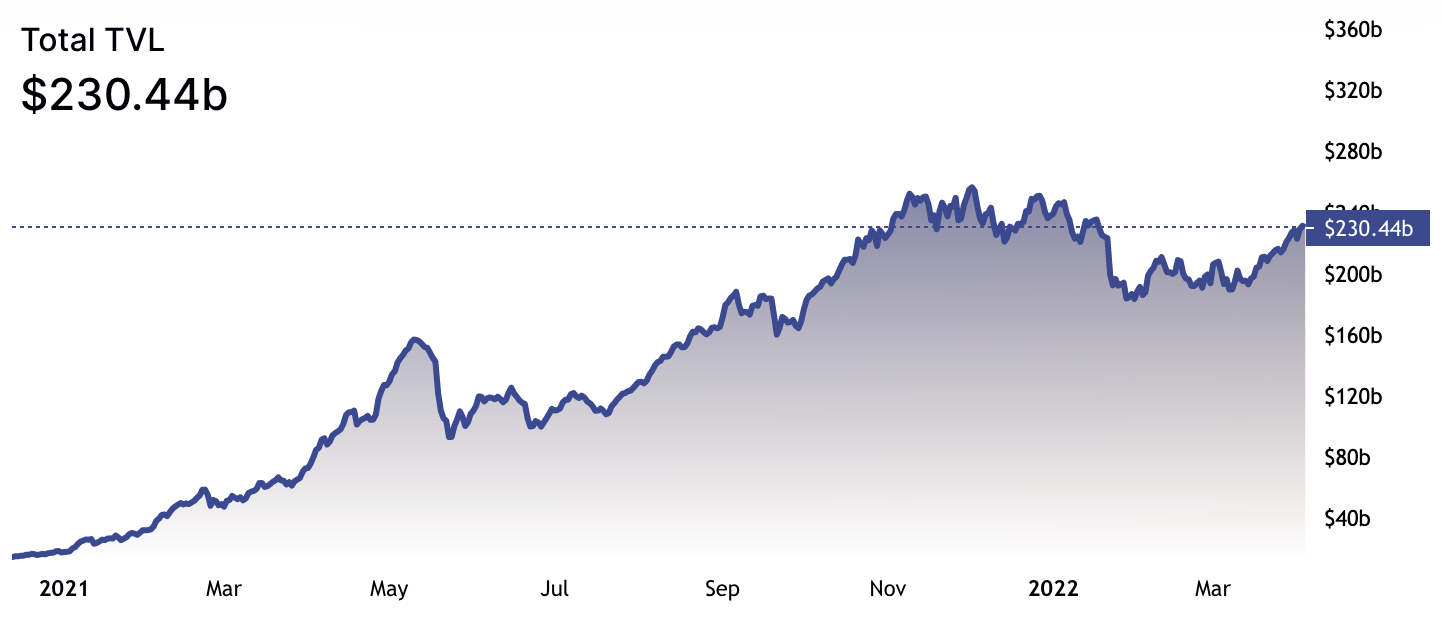
\includegraphics[width=100mm,scale=0.5]{figures/01-introduction-defi-lama.png}
    \caption[Fig 1]{\href{https://defillama.com/}{DeFi Llama}, DeFi industry analyst.\label{fig:defi-tvl}}
  \end{center}
\end{figure}

This meteoric rise reflects the speed with which individuals, traders, companies, and other groups have identified the opportunities and advantages created by DeFi. For example:
\begin{itemize}
\item Protecting individuals’ privacy while accessing financial services.
\item Eliminating unnecessary intermediaries.
\item Cutting out human foul play with smart contracts.
\item Trustless and decentralized architecture.
\end{itemize}

However, for all the good it brings, DeFi has also caught the attention of two other groups:
\begin{enumerate}
\item Bad actors, e.g., organized crime and terrorist groups, and insider traders
\item Regulators
\end{enumerate}
The same characteristics that make DeFi attractive to legitimate individuals and organizations also attract the worst aspects of humanity—and the organizations set up to protect against them.

\subsection{DeFi Attracts Unwanted Attention Due to Lack of KYC and AML}

The simple fact is that criminals and other bad actors thrive in economic environments that lack adequate controls to identify and exclude them. This is why organizations like the Financial Action Task Force (FATF) exist—to advise regulators on the policies needed to (as far as possible) cut bad actors out of their financial systems.

FATF—an intergovernmental group founded on the initiative of the G7 summit in 1989—produced the original recommendations for Anti-Money Laundering (AML) regulations in 1990. The regulations that sprang from these recommendations were bolstered by the 2001 Patriot Act following the 9/11 terrorist attacks, which coined the term KYC: Know Your Customer. FATF has updated its recommendations several times in the intervening years. Today, most countries employ some version of the group’s recommended AML and KYC regulations.

However, so far, DeFi has been minimally affected by regulation. While some individual DeFi protocols operate basic KYC checks, they typically aren’t well implemented and don’t significantly impede bad actors. Worse, due to poor implementation, they often place users’ personal data at risk and run contrary to the privacy principles of DeFi.

Given the explosion of interest—and capital—in DeFi protocols, the ecosystem has inevitably attracted the attention of bad actors and regulators.

\subsection{What Problems Does a Lack of KYC/AML Cause?}
Beyond attracting unwanted attention, DeFi’s lack of KYC and AML creates three huge problems:

\begin{enumerate}
\item \textbf{It keeps big players out of the ecosystem}\\
Currently, many regulated market makers are effectively shut out of the DeFi ecosystem. While DeFi doesn’t yet have strong regulations, these organizations \emph{do}—and that means they can’t engage in any trades without knowing who their counterparties are.

\item \textbf{It limits liquidity}\\
The exclusion of major market makers means less liquidity in the ecosystem and therefore fewer money-making opportunities for everybody.

\item \textbf{It harms trust in DeFi trading}\\
It isn’t possible to interact through a DeFi marketplace with the assurance that counterparties aren’t bad actors. Since most individuals and organizations would prefer not to trade with criminals or terrorists, this uncertainty undoubtedly impacts DeFi’s reputation—and possibly its uptake.

\end{enumerate}

\subsection{Regulations are Imminent}
There is no doubt that KYC and AML regulations for DeFi are imminent. Some self-proclaimed DeFi providers may already fall under FATF’s revised definition of a Virtual Asset Service Provider (VASP). FATF guidance from October 2021 notes that:

\begin{figure}[htbp]
\begin{quote}
\centering
"[...] creators, owners and operators or some other persons who maintain control or sufficient influence in the DeFi arrangements [...] may fall under the FATF definition of a VASP where they are providing or actively facilitating VASP services."
\caption{FATF, \href{https://www.fatf-gafi.org/publications/fatfrecommendations/documents/guidance-rba-virtual-assets-2021.html}{Updated Guidance} for a Risk-Based Approach to Virtual Assets and Virtual Asset Service Providers~\cite{fatf-guidance}.\label{cap:fatf-guidance}}
\end{quote}
\end{figure}

This would make them subject to the infamous \emph{Travel Rule}, which requires the collection of identifying information on the originators and beneficiaries of domestic and cross-border wire transfers—including names, account numbers, and physical addresses.

Again, while FATF guidance isn’t immediately binding, regulators worldwide take it seriously—and it is usually enshrined in law by most developed nations in close to unchanged form.

The facts are simple: DeFi regulation is coming—initially as KYC/AML requirements, but ultimately in the form of regulations designed to protect investors (e.g., from insider trading) and block bad actors in a similar manner to that used in traditional financial markets.

\subsection{Protecting Core DeFi Values}
Given that regulation is inevitable, the aim should be to identify a solution that satisfies dApps’ new regulatory requirements \emph{without} hindering basic DeFi values of privacy and decentralization.

\begin{tcolorbox}[width=\textwidth,colback={light-gray},title={\textbf{Privacy vs. Anonymity (and Why it Matters)}},colbacktitle=light-gray,coltitle=black]
It’s a popular misconception that DeFi allows individuals to trade anonymously. Blockchain as a whole at best offers pseudo-anonymity. Since wallet IDs remain constant, users must constantly protect against their identities being linked to a wallet address—something that would typically be trivial for a government agency.

In practice, well-designed dApps provide individuals with privacy. It is typically possible to trade between counterparties without either side knowing the identity of the other. This privacy component of DeFi must be protected when seeking solutions to upcoming regulations.
\end{tcolorbox}

This white paper proposes the Gateway Protocol as a solution to allow dApps to meet upcoming KYC and AML requirements without:

\begin{enumerate}
\item Developing user verification capabilities internally.
\item Viewing or holding any personal information on users.
\item Directly interacting with regulators in most cases.
\end{enumerate}

In doing so, the Gateway Protocol will protect DeFi users’ privacy while enabling the positive impact of upcoming regulations. Similarly, the Gateway Protocol operates as a DAO and is governed via a voting system that anyone can join, ensuring the solution remains as decentralized as possible.

\subsection{Benefits for the DeFi Community}

By addressing the needs of regulators while protecting DeFi values, the Gateway Protocol will benefit all DeFi stakeholders:
\begin{itemize}
\item \textbf{Regulators} can ensure bad actors are (as far as possible) excluded from the DeFi ecosystem.
\item \textbf{dApps} can adhere to new KYC/AML regulations without developing those capabilities internally.
\item \textbf{Regulated institutions} can join the DeFi ecosystem while satisfying existing KYC/AML regulations.
\item \textbf{Legitimate DeFi adopters} can trade freely without worrying that counterparties may be bad actors.
\item \textbf{All DeFi stakeholders} can benefit from increased liquidity and reduced influence of bad actors such as criminal and terrorist groups and insider traders.
\end{itemize}
